\begin{center}
\makeatletter
\@ifundefined{color@atlasink}{\definecolor{atlasink}{HTML}{33312E}}{}
\@ifundefined{color@atlasgray}{\definecolor{atlasgray}{HTML}{9A958C}}{}
\@ifundefined{color@atlasblue}{\definecolor{atlasblue}{HTML}{2E6F9E}}{}
\@ifundefined{color@atlasgreen}{\definecolor{atlasgreen}{HTML}{4C8C3F}}{}
\@ifundefined{color@atlasred}{\definecolor{atlasred}{HTML}{C0473B}}{}
\@ifundefined{color@atlasgold}{\definecolor{atlasgold}{HTML}{D69A2A}}{}
\@ifundefined{atlascaption}{%
  \newcommand{\atlascaption}[3]{\shortstack{\footnotesize Figure~#1. \textbf{#2:}\\#3}}%
}{}
\@ifundefined{glowstroke}{%
  \newcommand{\glowstroke}[3]{%
    \draw[#1, line width=1.5pt, line cap=round]
      plot[domain=#2,samples=100,smooth] (\x,{#3});%
  }%
}{}
\makeatother
\tikzset{
  atlas axes/.style={atlasink, line width=0.7pt, line cap=round, ->},
  atlas curve/.style={line width=1.5pt, line cap=round, line join=round},
  dropline/.style={atlasgray, line width=0.6pt, dash pattern=on 2pt off 2pt},
  atlas dot/.style={fill=atlasink, draw=white, line width=0.4pt, circle, inner sep=0pt, minimum size=4.2pt},
}

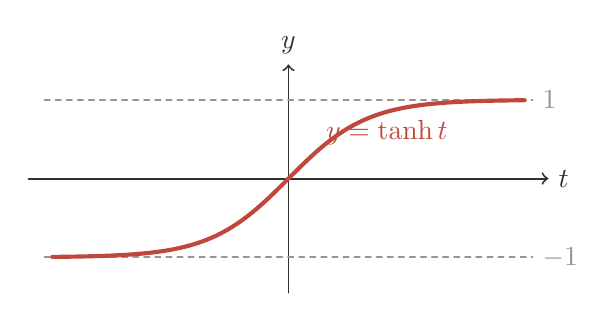
\begin{tikzpicture}[scale=1.0, line cap=round, line join=round]
  \draw[atlas axes] (-3.3,0)--(3.3,0) node[right] {$t$};
  \draw[atlas axes] (0,-1.45)--(0,1.45) node[above] {$y$};
  \draw[dropline] (-3.1,1)--(3.1,1) node[right] {$1$};
  \draw[dropline] (-3.1,-1)--(3.1,-1) node[right] {$-1$};
  \glowstroke{atlasred}{-3:3}{(exp(\x)-exp(-\x))/(exp(\x)+exp(-\x))}
  \node[atlasred] at (1.25,0.58) {$y=\tanh t$};
\end{tikzpicture}

\atlascaption{H4}{Hyperbolic tangent}{Odd, increasing, with horizontal asymptotes $y=\pm 1$.}
\end{center}


\begin{definitionbox}{Definition}
\begin{definition}[Hyperbolic tangent]
\label{def:hyperbolic-tangent}
For each $t\in\mathbb{R}$, define the \emph{hyperbolic tangent} by
\[
  \tanh t=\frac{\sinh t}{\cosh t}.
\]
\end{definition}
\end{definitionbox}
\begin{remark*}[Domain and range]
The function $\tanh$ is defined on all of $\mathbb{R}$ because
$\cosh t\geq 1$. Its range is $(-1,1)$.
\end{remark*}
\begin{dependencies}
\begin{itemize}
  \item \hyperref[def:hyperbolic-sine]{Hyperbolic sine}
  \item \hyperref[def:hyperbolic-cosine]{Hyperbolic cosine}
\end{itemize}
\end{dependencies}
